\chapter{Global Settings}
\label{global}

\section{Play Modes}
\label{legato}

Odin 2 is capable of three play modes: \fat{Polyphonic}, \fat{Legato} and \fat{Retrig}.

\vspace{3mm}
In the default mode \fat{Poly}, you can play up to 24 voices. When you reached the voice limit, the oldest note that is not still held down will be stolen and used as the new voice.

\vspace{3mm}
In \fat{Legato} mode, you have only one voice to play with. When playing another note while still holding down the last note, \fat{the envelope generators (see \ref{ADSR}) will not be retriggered}. 
This essentially creates one long note, which changes pitch as you press the second key. Legato mode can be very useful if you don't want notes to overlap, for example in a lead or bass type of sound. 

\vspace{3mm}
\fat{Retrig} mode also features a single voice. In contrast to Legato mode, the envelopes perform a \fat{soft-reset} when overlapping notes are triggered. In that case, the Attack section of the envelopes (see \ref{ADSR})
is not started from zero, but the value it is currently on. This creates a smooth transition between the two notes, while still giving each note their own percussive start.

\vspace{3mm}
The drop-down to select the play mode can be found on the top of the GUI.


\audioparameter{Play Mode}{0}{0}{
    \begin{center}
        
\includegraphics[width=0.15\textwidth]{graphics/poly_legato.png}
    \end{center}
    Select between playmodes \fat{Poly}, \fat{Legato} and \fat{Retrig}.
}

\clearpage
\section{Unison}
\label{unison}

\begin{center}
    
\includegraphics[width=0.4\textwidth]{graphics/unison.png}
\end{center}

The Unison feature makes it possible to trigger a stack of voices together instead of a single voice. These voices can be slightly detuned and spread over the stereo field, to generate a much wider, bigger sound. While detune and width parameters are available as dedicated controls, you can modulate any parameter for each unison voice independently with the modulation destination "Unison Index" (see Section \ref{mod_destinations}).

\vspace{3mm}
The controls for Unison can be found in the top-left corner of the GUI.

\vspace{3mm}
\begin{tcolorbox}[colback=yellow!10!white,
        colframe=white!20!black,
        center,
        valign=top,
        halign=left,
        center title,
        width=\textwidth]

    Since the implementation of Unison in Odin 2 literally triggers multiple voices, using high Unison counts uses lots of CPU time. Use it with care, if you run into performance issues, you can always bounce the track to audio in your DAW.
\end{tcolorbox}

\audioparameter{Unison Count}{0}{0}{
    Determines how many voices are triggered when you press a button. 

    Try to keep the Unison Count low if you're experiencing performance issues.
}

\audioparameter{Unison Detune}{0}{1}{
    Controls the amount of detune for the voices in the unison stack.
}

\audioparameter{Unison Width}{0}{1}{
    Controls the stereo spread of the voices in the unison stack. Having this value at zero will put all voices in the center of the stereo field. Having the value at one puts the first voices hard-left and the last on hard-right. The voices inbetween are spread linearly inbetween
}

\section{Microtuning}
\label{microtuning}

Starting from version 2.3, Odin 2 supports microtuning. This feature can be used from subtle changes, like retuning the instrument to a different base frequency to a complete remapping of the keyboard.
You can find the Tuning dropdown on top of the GUI:

\begin{center}
    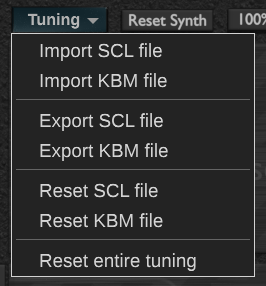
\includegraphics[width=0.3\textwidth]{graphics/microtuning.png}
\end{center}

The tuning is specified by two separate files: The \fat{keyboard mapping} files (\fat{.kbm}) and \fat{Scala} files (\fat{.scl}). Together, they make up a complete and arbitrary tuning of the synthesizer.
To read up on the specifications, use these resources:

\vspace{3mm}
Scala File Specification: \url{http://www.huygens-fokker.org/scala/scl_format.html}

\vspace{3mm}
Keyboard Mapping Specification: \url{http://www.huygens-fokker.org/scala/help.htm#mappings}

\vspace{3mm}
A large variety of tuning files can be downloaded from this scale archive: \url{http://www.huygens-fokker.org/docs/scales.zip}.

\vspace{3mm}
To generate your own .kbm and .scl files, use the "Export SCL/KBM file" option. This will let you save the currently used files and adjust them as needed. You can then import the modded file again.









\section{Glide and Master}
\label{glide}

The last two remaining parameters, Glide and Master are located in the bottom left corner of the GUI.

\begin{center}
    
\includegraphics[height=0.2\textwidth]{graphics/master_glide.png}
\end{center}

\audioparameter{Glide}{1}{1}{
    Makes the pitch of newly triggered voices glide from the frequency of the last note to the frequency of the current note. The glide curve is exponential.
}

\audioparameter{Master}{1}{1}{
    Controls the output gain of the synthesizer.
}
